\section{Auswertung}
\label{sec:Auswertung}

\subsection{Errechnete Theoriewerte}

Mit Hilfe der gemessenen Daten und Gleichungen \ref{eq:zyl1} und \ref{eq:zyl2}
lassen sich die Trägheitsmomente der beiden Zylinder
als

\begin{equation*}
  I=0,787 \cdot 10^{-3}\,\si[inter-unit-product=\cdot]{\kilo\gram\meter\squared}
\end{equation*}

\noindent und als

\begin{equation*}
  I=15,432 \cdot 10^{-3}\,\si[inter-unit-product=\cdot]{\kilo\gram\meter\squared}
\end{equation*}

\noindent berechnen. Bei der Puppe wird zusätzlich 
Gleichung \ref{eq:Kugel} und der Satz von Steiner \ref{eq:steiner}
benötigt. Für die erste Position ergibt sich ein
Trägheitsmoment von

\begin{equation*}
  I=7,916 \cdot 10^{-5}\,\si[inter-unit-product=\cdot]{\kilo\gram\meter\squared}
\end{equation*}

\noindent und für die zweite ein Trägheitsmoment von

\begin{equation*}
  I=1,591 \cdot 10^{-5}\,\si[inter-unit-product=\cdot]{\kilo\gram\meter\squared}
\end{equation*}

\noindent Dabei wurde die Dichte des Holzes der Puppe
als $670\,\si{\kilo\gram \per \cubic \meter}$ (siehe \cite{holz})
angenommen.
















\subsection{Bestimmung der Winkelrichtgröße und des Eigenträgheitsmoments der Drillachse}

Die Winkelrichtgröße D lässt sich mithilfe der Gleichungen (5 und 7) berechnen. Im Versuch standen 
Kraftarm $\vec{r}$ und Kraft $\vec{F}$ senkrecht zueinander, wodurch der Betrag von Gleichung (5) 
zu
\begin{equation}
    M = F \cdot r
    \label{eq:ae1}
\end{equation}
\noindent
wird. Werden nun (7) und \ref{eq:ae1} gleichgesetzt und nach D umgestellt, ergibt sich die Gleichungen
\begin{equation}
    D = \frac{F\cdot r}{\phi}.
    \label{eq:ae2}
\end{equation}
\noindent
Mit den Werten aus der Tabelle \ref{eq:a1}, der Formel \ref{eq:ae2} und den allgemeinen Formeln für den Mittelwert
\begin{equation}
    \bar{x} = \frac{1}{N} \sum_{n=1}^N x_n 
    \label{eq:ae3}
\end{equation}
\noindent
und der Standartabweichung
\begin{equation}
    \sigma = \sqrt{\frac{1}{N(N-1)} \sum_{n=1}^N (x_n - \bar{x})^2}
\end{equation}
\noindent
ergibt sich für die Winkelrichtgröße D der Wert D = $(0.017027 \pm 0.001539)\,$Nm.

\begin{table}[H]
\normalsize

\centering
\sisetup{table-format=4.0}
\begin{tabular}{c c}
\toprule
    $\phi$\,/\, rad & $F$\,/\,$\si{\newton}$ \\
    \midrule

$\pi/6$  &   0.02   \\
$\pi/3$  &   0.12   \\
$\pi/2$  &   0.21   \\
$2\pi/3$ &   0.31   \\
$5\pi/6$ &   0.40   \\
$\pi$    &   0.50   \\
$7\pi/6$ &   0.60   \\
$4\pi/3$ &   0.70   \\
$3\pi/2$ &   0.80   \\
$5\pi/3$ &   0.90   \\ 

    \bottomrule
\end{tabular}
\caption{Aufgenommene Werte zur Bestimmung der Winkelrichtgröße D}
\label{tab:a1}
\end{table}

















\noindent
Um das Eigenträgheitsmoment $I_D$ bestimmen zu können, ist es zuerst notwendig das gesamte 
Trägheitsmoment des in \ref{fig:b} zu sehenden Aufbaus zu berechnen. Dieses setzt sich mithilfe 
des Satzes von Steiner zu dem Ausdruck
\begin{equation}
    I_{ges} = I_D + 2\cdot I_{zh} + 2\cdot m_{zh} \cdot a^2
\end{equation}
\noindent
zusammen. Dabei gibt $I_{zh}$ das Trägheitsmoment eines senkrecht zu der Drehachse liegenden Zylinders an, 
welches sich über 
\begin{equation}
    I_{zh} = m_{zh} \cdot \Big( \frac{R^2}{4} + \frac{h^2}{12} \Big)
\end{equation}
\noindent
berechnen lässt (Verweis auf Versuchsanleitung). Dieses Zwischenergebnis lässt sich nun in die 
quadrierte Gleichung (REFERENZ) einsetzen, wodurch sich 
\begin{equation}
    T^2 = \frac{4 \pi^2 I_D}{D} + \frac{8 \pi^2 m_{zh}}{D} \cdot a^2 + \frac{8 \pi^2 m_{zh} R^2}{4 D} + \frac{8 \pi^2 m_{zh} h^2}{12 D} 
\end{equation}
\noindent 
ergibt. Der Ausdruck hat die Form der allgemeinen Geradengleichung
\begin{equation}
    y(x) = m\cdot x + b
\end{equation}
\noindent
wobei 
\begin{equation}
    m = \frac{8 \pi^2 m_zh}{D}
\end{equation}
und 
\begin{equation}
    b = \frac{4 \pi^2 I_D}{D} + \frac{8 \pi^2 m_{zh} R^2}{4 D} + \frac{8 \pi^2 m_{zh} h^2}{12 D}
    \label{eq:b}
\end{equation}
gilt. Über die lineare Regression ergeben sich $m = (673.436 \pm 31.466)\,\frac{\si{\second}^2}{\si{\meter}^2}$ und $b = (8.064 \pm 1.870)\,\si{\second}^2$ als gesuchte Werte.
Wird nun \ref{eq:b} nach dem Eigenträgheitsmoment $I_D$ aufgelöst
\begin{equation}
    I_D = \frac{b D}{4 \pi^2} - \frac{m_{zh} R^2}{2} - \frac{m_{zh} h^2}{6}
\end{equation}
\noindent
lässt sich durch die gaußsche Fehlerfortpflanzung
\begin{equation}
    \sigma_f = \sqrt{\sum_{i=1}^m   \Big(   \frac{\partial f}{\partial x_i} \Big)^2 \sigma_{x_{i}}^2       }
\end{equation}
\noindent
als Wert für das Eigenträgheitsmoment $I_D$ der Wert $I_D = (0.024 \pm 0.006)\, \si{\kg}\,\si{\meter}^2$.




\begin{figure}
    \centering
    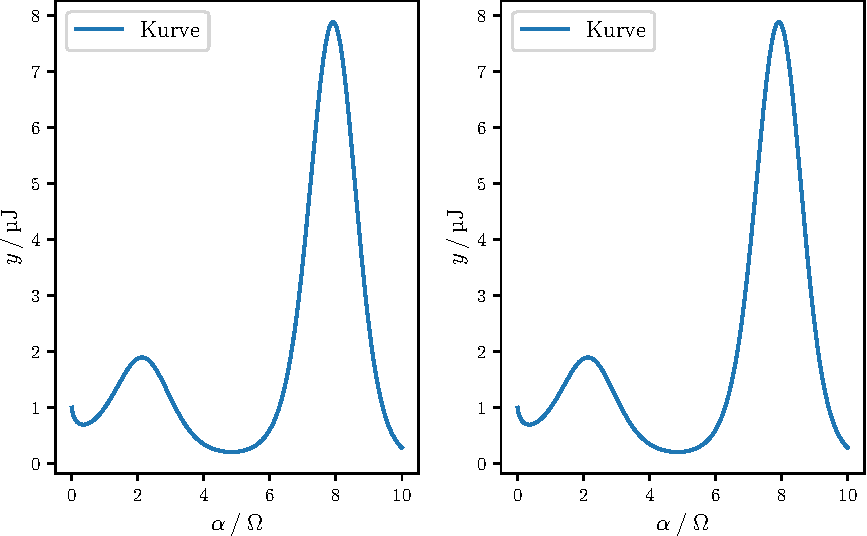
\includegraphics[width=10cm]{build/plot.pdf}
    \caption{Darstellung der Messwerte und der linearen Regression zur Bestimmung des Eigenträgheitsmoments $I_D$}
\end{figure}


\begin{table}[H]
\normalsize

\centering
\sisetup{table-format=4.0}
\begin{tabular}{c c c c}
\toprule
    $a$\,/\,$\si{\meter}$ &  $T$\,/\,$\si{\second}$ & $a^2$\,/\,$\si{\meter}^2$ &  $T^2$\,/\,$\si{\second}^2$ \\
    \midrule

0.30  &   8.35 &  0.0900      & 69.7225\\
0.285 &   7.73 &  0.0812  & 59.7529\\
0.27  &   7.65 &  0.0729    & 58.5225\\
0.255 &   7.13 &  0.0650  & 50.8369\\
0.24  &   6.83 &  0.0576    & 46.6489\\
0.225 &   6.60 &  0.0506  & 43.5600\\
0.21  &   6.40 &  0.0441    & 40.9600\\
0.195 &   5.84 &  0.0380  & 34.1056\\
0.18  &   5.24 &  0.0324    & 27.4576\\
0.165 &   5.06 &  0.0272  & 25.6036\\ 

    \bottomrule
\end{tabular}
\caption{Aufgenommene Werte zur Bestimmung des Eigenträgheitsmoments $I_{D}$ der Drillachse (Auslenkung betrug 15°)}
\label{tab:a2}
\end{table}





\subsection{Berechnung der Trägheitsmomente von zwei Körpern}

\subsubsection{Trägheitsmoment eines kurzen Zylinders}

Das Träheitsmoment eines Vollzylinders, der sich um seine Symmetrieachse dreht ist durch 
Gleichung (Verweis) gegeben. Die in Tabelle \ref{tab:a4} aufgeführten Werte wurden bei einer 
Auslenkung von $\phi = 15\,°$ aufgenommen. Mit dem Wert $T_{K1} = 1.032 \pm 0.0463\, \si{\second}$
für die Periodendauer lässt sich über die nach $I$ umgestellte Gleichung (VERWEIS)
\begin{equation}
    I = \frac{T^2 D}{4 \pi^2}
\end{equation}
und der Gaußsche Fehlerfortpflanzungformel (VERWEIS)
\begin{equation} 
    \Delta I_{K1} = \sqrt{\frac{T_{K1}^2 D^2}{4 \pi^4}\Delta T_{K1}^2 + \frac{T_{K1}^4}{16 \pi^4}\Delta D^2} 
\end{equation}



\begin{table}[H]
\normalsize

\centering
\sisetup{table-format=4.0}
\begin{tabular}{c c}
\toprule
    Messung  & $T$\,/\,$\si{\second}$ \\
    \midrule

1  &   0.92   \\
2  &   1.16   \\
3  &   0.96   \\
4  &   1.12   \\
5  &   1.00   \\

    \bottomrule
\end{tabular}
\caption{Aufgenommene Werte zur Bestimmung des Trägheitsmoments}
\label{tab:a4}
\end{table}













Siehe \autoref{fig:plot}!
>>>>>>> ed2895cb6604afe0ad298a0bfca18f1470dafd42
